\chapter{Extended Tables \& Figures}
\label{app:a}

\begin{table}[]
  \vspace{-2cm}
\captionof{table}{Basic experiment hyper parameters}
\label{tab:base}
% \begin{tabularx}{p{.2\linewidth}l p{.7\linewidth}}
  \renewcommand{\arraystretch}{1.15}
\small
\begin{tabularx}{1.1\linewidth}{ll X}
Hyperparameter                  & Value             & Description                                                                                              \\
  \hline
mini-batch size                 & 32                & Number of random samples for each stochastic gradient descent update                                     \\
replay memory size              & $10^6$            & Replay memory contains this number of most recent frames for SGD updates                                 \\
agent history length            & 4                 & Number of most recent frames used as input to the Q network                                              \\
target network update frequency & 2000*             & Every 2000 parameter updates the target network gets updated with the parameters of the current network. \\
discount factor                 & 0.95              & Discount $\gamma$ used in Q-learning update                                                              \\
frame skip                      & 4                 & The agent only sees every 4th frame                                                                      \\
update frequency                & 1                 & Parameter updates occur every action selection                                                           \\
learning rate                   & $2 \cdot 10^{-4}$ & Learning rate $\eta$ used by RMSProp                                                                     \\
RMS decay                       & 0.99              & Gradient moving average decay factor $\rho$ for RMSProp                                                  \\
RMS epsilon                     & $10^{-6}$         & RMSProp small stability value added to denominator (see \ref{eq:rmsprop})                              \\
clip delta                      & false             & Whether to clip the delta; \cite{Mnih2015} clips this to $[-1, 1]$                                      \\
initial exploration             & 1                 & Initial value for $\epsilon$ in $\epsilon$-greedy                                                        \\
final exploration               & 0.1               & Smallest value for $\epsilon$ in $\epsilon$-greedy                                                       \\
epsilon decay                   & $10^{-6}$         & $\epsilon$ decays linearly over this amount of actions                                                   \\
replay start size               & 100               & Wait with training until the replay memory contains at least this amount of frames                       \\
max no-ops                      & 10**              & Start with a random amount of no-ops that is at most this amount                                         \\
resize frame method             & scale***          & Processing step employed to resize frames in order to reduce amount of pixels                            \\
\end{tabularx}
\paragraph{}
  The values in this table are based entirely on the DQN implementation by
  \cite{Mnih2013},
  except for those annotated.

  \textbf{*} The original implementation employs no separate target network.
  This is added in for stability.

  ** The original implementation uses no initial no-ops.
  This is added in to add some stochasticity to the games.

  *** The original implementation crops out the required area from a frame.
  This does not generalize well to games where important information
  falls outside of this frame.
\end{table}

\begin{table}
  \captionof{table}{\textit{Boost} experiment hyper parameters}
  \label{tab:boost}
  \renewcommand{\arraystretch}{1.3}
\begin{tabularx}{1.\linewidth}{ll X}
Hyperparameter                  & Value             & Description                                                                                              \\
  \hline
discount factor                 & 0.99              & Discount $\gamma$ used in Q-learning update                                                              \\
update frequency                & 4                 & Parameter updates occur every action selection                                                           \\
replay start size               & 50000               & Wait with training until the replay memory contains at least this amount of frames                       \\

\end{tabularx}

\paragraph{}
\small
The rest of the parameters not present here are as supplied by Table \ref{tab:base}.
The combination in this table is gotten from \cite{Mnih2015},
which tended to work well for some games and considerably sped up training
because less updates are performed.

It is however sufficient for comparisons.
\end{table}

\begin{table}
  \captionof{table}{\textit{LSTM} basic parameters}
  \label{tab:lstm_params}
  \renewcommand{\arraystretch}{1.3}
\begin{tabularx}{1.\linewidth}{ll X}
Hyperparameter                  & Value             & Description                                                                                              \\
  \hline
nonlinearity & tanh & Nonlinearity applied to output \\
gradient clipping & 10 & Gradients are clipped to 10 \\
\end{tabularx}

\paragraph{}
All gates are constructed with all weights initialized randomly
according to a normal distribution with standard deviation $0.1$.
They all apply a sigmoid nonlinearity to their output.

The cell state unit has its weights initialized likewise
except for the cell state value which gets initialized to 0.
A tanh nonlinearity is applied to the output of this unit.
\end{table}

\begin{figure}[htpb]
  \centering
  \captionof{figure}{Comparison of basic DQN network performance}
  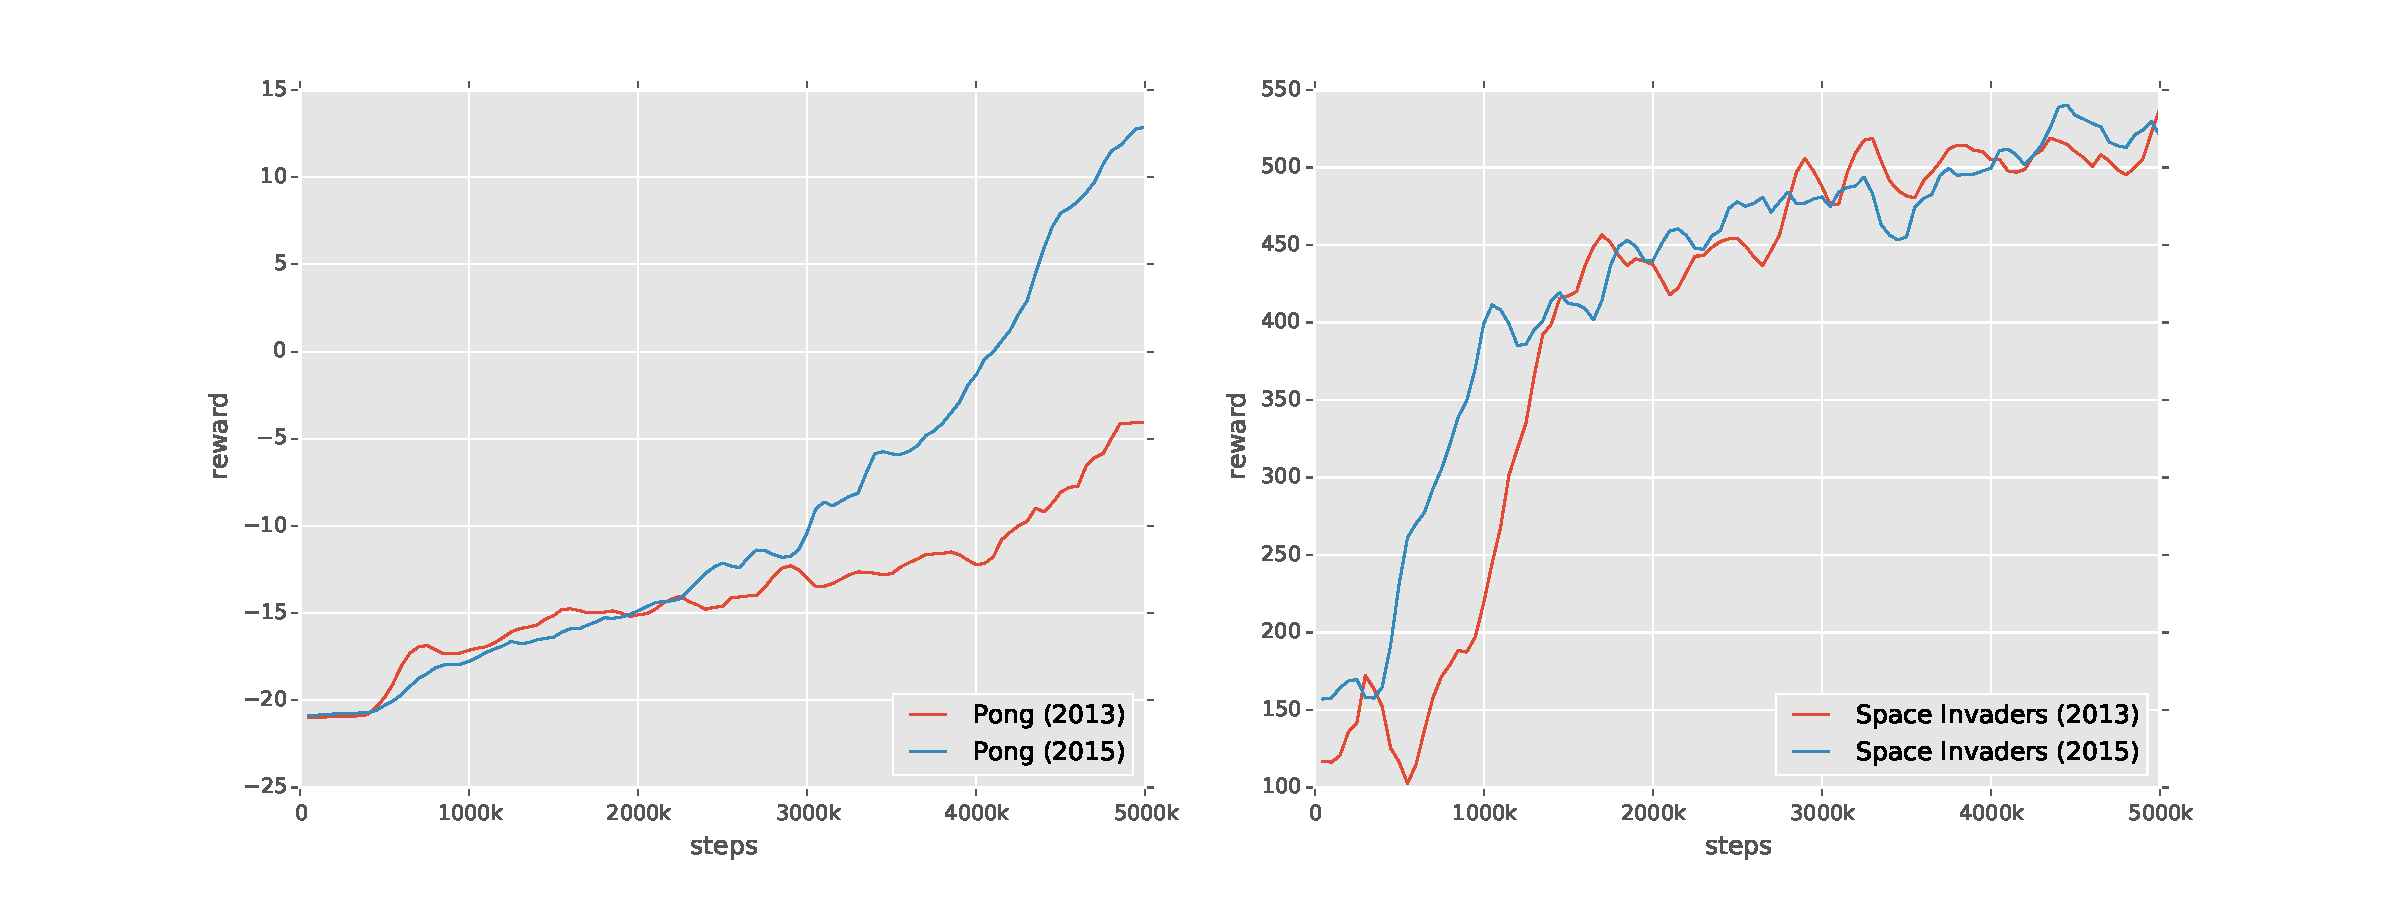
\includegraphics[width=1.0\linewidth]{nips_vs_nature_rewards.pdf}
  \raggedright
  \paragraph{}
    A comparison of learning curves for the two architectures described in
    \cite{Mnih2013} and \cite{Mnih2015}
    with network structure depicted in Figure \ref{fig:dqn_networks}
    and parameters in Table \ref{tab:boost}.

    Some games benefit more from increased network capacity than others.
  \label{fig:nips_vs_nature_rewards}
\end{figure}

\begin{figure}[]
  \paragraph{}
  Each experiment is run 3 times
  except the basic DQN experiments which are all run 5 times
  (no matter whether 1 or 4 frames as input).
  An experiment is run over 100 epochs of each 50000 steps.
  After each epoch a test phase takes place to calculate gathered rewards
  over 10000 steps.
  These are then averaged and represent a single point.
  The average Q-values are calculated over 3200 states
  that are randomly gathered at the start of the experiment.

  \paragraph{}
  Where rewards or average Q-values are illustrated in a graph,
  the graph is smoothed with a weighted running average
  with a window of 5
  to increase visibility.

  \paragraph{}
  Where the Wilcoxon signed-rank test is applied,
  it tests the null hypothesis that the samples
  are drawn from the same distribution.

  \caption{Basic experiment setup}
  \label{fig:basic_setup}
\end{figure}

\begin{table}
  \center
  \renewcommand{\arraystretch}{1.3}
  \begin{tabular}{lrrrrrr}
\hline
           &   (3,2) &   (2,2) &   (3,1) &   (2,2) RGB &   (2,3) &   DQN-4 \\
\hline
 (3,2)     &    1    &    0.83 &    0.83 &        0.05 &    0.66 &    0.51 \\
 (2,2)     &    0.83 &    1    &    0.51 &        0.05 &    0.19 &    0.05 \\
 (3,1)     &    0.83 &    0.51 &    1    &        0.05 &    0.28 &    0.05 \\
 (2,2) RGB &    0.05 &    0.05 &    0.05 &        1    &    0.05 &    0.05 \\
 (2,3)     &    0.66 &    0.19 &    0.28 &        0.05 &    1    &    0.38 \\
 DQN-4     &    0.51 &    0.05 &    0.05 &        0.05 &    0.38 &    1    \\
\hline
\end{tabular}
  \caption[Statistical results for 3D Conv]{
    Wilcoxon signed-rank test p-values
    for the time to a reward of 10
    for the 3D convolutional architectures
    on the game Pong.
  }
  \label{tab:conv3d_wilcoxon}
\end{table}


\begin{table}
  \center
  \renewcommand{\arraystretch}{1.3}
  \begin{tabular}{lrrrr}
\hline
                 &   LF shared &   LF separate &   LF shared (RGB) &   DQN-4 \\
\hline
 LF shared       &        1    &          0.28 &              0.05 &    0.19 \\
 LF separate     &        0.28 &          1    &              0.05 &    0.05 \\
 LF shared (RGB) &        0.05 &          0.05 &              1    &    0.05 \\
 DQN-4           &        0.19 &          0.05 &              0.05 &    1    \\
\hline
\end{tabular}
  \caption[Statistical results for Late Fusion]{
    Wilcoxon signed-rank test p-values
    for the time to a reward of 10
    for the Late Fusion architectures
    on the game Pong.
  }
  \label{tab:lf_wilcoxon}
\end{table}


\begin{table}
  \center
  \begin{tabular}{lrrrrr}
\hline
               &   3D Conv &   LF &   3D Conv (RGB) &   LF (RGB) &   DQN-4 \\
\hline
 3D Conv       &      1    & 0.05 &            1    &       0.05 &    0.05 \\
 LF            &      0.05 & 1    &            0.05 &       0.05 &    0.05 \\
 3D Conv (RGB) &      1    & 0.05 &            1    &       0.05 &    0.05 \\
 LF (RGB)      &      0.05 & 0.05 &            0.05 &       1    &    0.05 \\
 DQN-4         &      0.05 & 0.05 &            0.05 &       0.05 &    1    \\
\hline
\end{tabular}
  \caption[Statistical results for comparing architectures]{
    Wilcoxon signed-rank test p-values
    for the time to a reward of 10
    for the best instances of each architecture
    on the game Pong.

    The LSTM architecture is left out because it
    never managed positive average scores.
  }
  \label{tab:lf_wilcoxon}
\end{table}


\begin{table}[htpb]
  \center
  \renewcommand{\arraystretch}{1.3}
  \begin{tabular}{ll}
\hline
 Architecture      & Steps to 10 reward                \\
\hline
 3D Conv           & $\num{1.6e+06} \pm \num{6.0e+04}$ \\
 Late Fusion (RGB) & $\num{1.1e+06} \pm \num{7.3e+04}$ \\
 3D Conv (RGB)     & $\num{1.0e+06} \pm \num{8.3e+04}$ \\
 Late Fusion       & $\num{2.6e+06} \pm \num{2.0e+05}$ \\
 DQN-4             & $\num{2.0e+06} \pm \num{2.9e+04}$ \\
\hline
\end{tabular}
  \caption[Time to threshold comparison]{
    Time to threshold
    of an accumulated reward of 10
    for Pong
    on the best instantiations of each architecture,
    excluding LSTM.
  }
\end{table}

\begin{figure}[htpb]
  \centering
  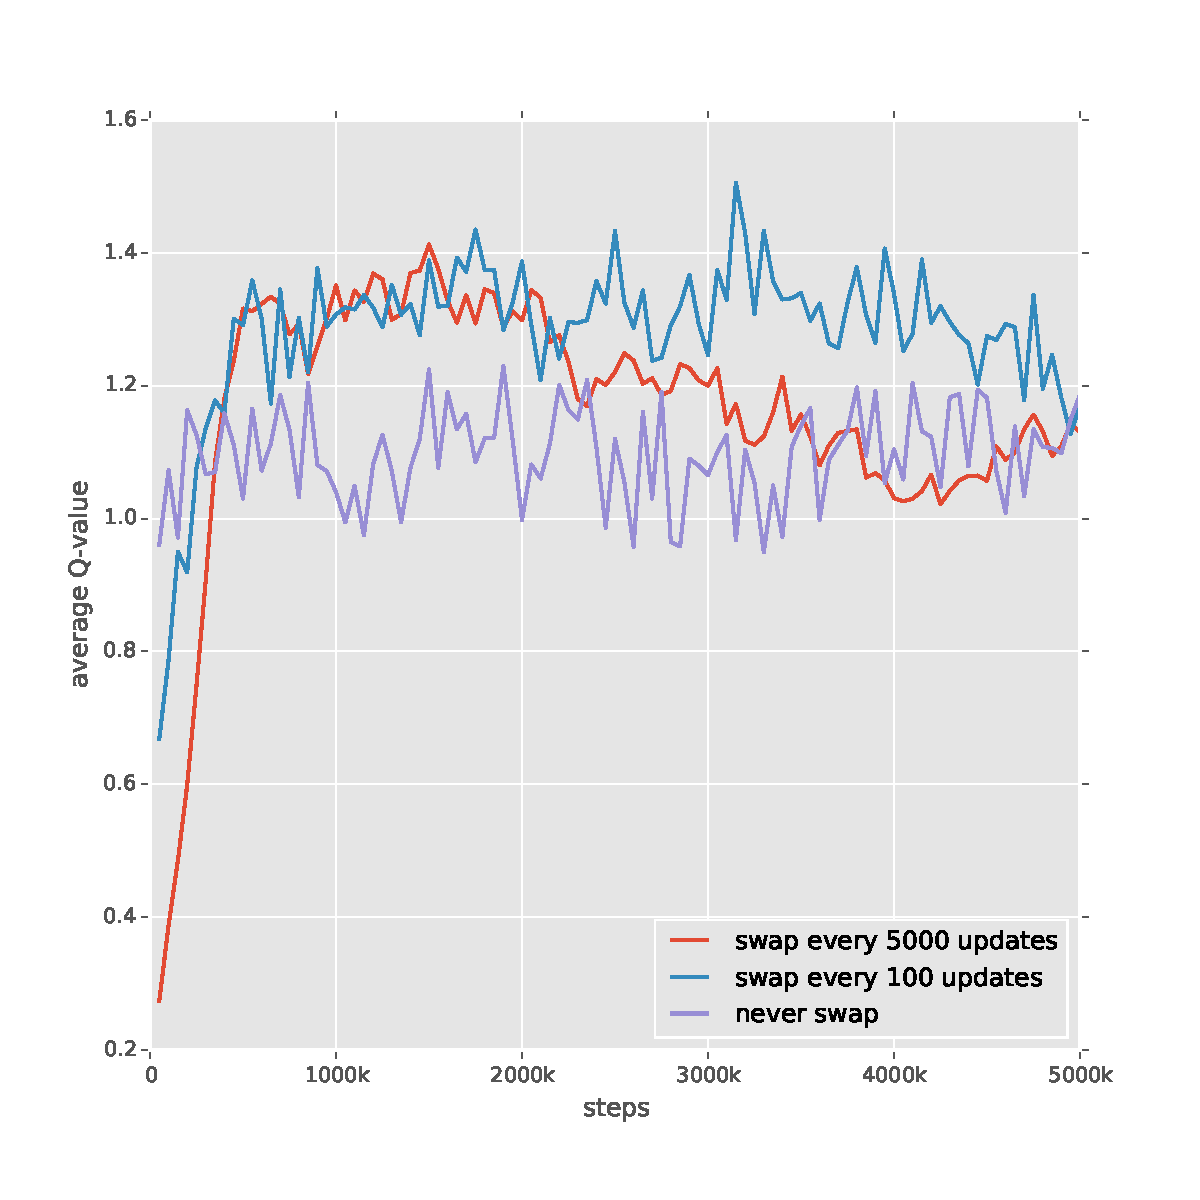
\includegraphics[width=0.6\linewidth]{freeze_qs.pdf}
  \caption[Target swap frequency comparison]{
    This graph depicts three runs of the game Space Invaders,
    each with a different interval for swapping
    the target Q-network,
    a measure that has been added to stabilize learning.

    The run that uses no separate target network
    does not really seem to learn any Q-values reliably
    while the network with the longest stable interval
    performs most least noisily
    and actually seems to learn values.
  }
  \label{fig:freeze_qs}
\end{figure}
